\documentclass[10pt,a4paper]{report}
\usepackage[utf8]{inputenc}
\usepackage[english]{babel}
\usepackage[T1]{fontenc}
\usepackage{amsmath}
\usepackage{amsfonts}
\usepackage{graphicx}
\usepackage{lmodern}
\usepackage{amssymb}
\usepackage{verbatim}
\usepackage{float}
\usepackage{minitoc}
\usepackage{amsthm}
\newtheorem{definition}{Definição}
\newtheorem{theorem}{Teorema}
\usepackage{hyperref}
\title{\LARGE{Software Security} \\ \vspace{0.5cm} \normalsize{Summary}}
\date{}

\begin{document}
\maketitle
\tableofcontents

\chapter{Language Based Security}
\section{Information Flow Security}
\subsection{Tracking Information Flow}
Perl has a taint mode feature that allows the tracking of input. When active all forms of input to the programs are marked as "tainted". Tainted variables taint variables explicitly calculated from them and tainted data may not be used in any sensitive command (with some exceptions).\\
\\
This mechanism implicits a set of security classes (tainted vs. untainted), as well as a classification of objects/information holders, a specification of when information can flow from onde security class to another and a way to determine security classes that safely represent the combination of two other.
\subsection{Information Flow Policies}
The goals of information security are confidentiality and integrity. Information flow policies specify how information should be allowed to flow between objects of each security class. To define one such policy we need:
\begin{itemize}
\item A set of security classes
\item A can-flow relation between them
\item An operator for combining them
\end{itemize}
\subsubsection{Information Flow Policies For Confidentiality}
Confidentiality classes determine who has the right to read and information can only flow towards confidentiality classes that are at least as secret.\\
\\
Information that is derived from the combination of two security classes takes a confidentiality classes that are at least as secret as each of them.
\subsubsection{Information Flow Policies For Integrity}
Integrity classes determine who has the right to write and information can only flow towards integrity classes that are no more trustful.\\
\\
Information that is derived from the combination of two integrity classes takes an integrity class that is no more trustful than each of them.
\subsubsection{Formal Information Flow Policies}
These policies can be described as a triple $(SC, \rightarrow, \oplus)$, where:
\begin{itemize}
\item $SC$ is a set of security classes
\item $\rightarrow \subseteq SC \times SC$ is a binary can-flow relation on $SC$
\item $\oplus: SC \times SC \rightarrow SC$ is an associative and commutative binary class-combining or join operator on $SC$
\end{itemize}
Example high-low policy for confidentiality:
\begin{itemize}
\item $SC = \{H,L\}$
\item $\rightarrow = \{(H,H), (L,L), (L,H)\}$
\item $H \oplus H = H, L \oplus H = H, L \oplus L = L$
\end{itemize}
And for integrity:
\begin{itemize}
\item $SC = \{H,L\}$
\item $\rightarrow = \{(H,H), (L,L), (H,L)\}$
\item $H \oplus H = H, L \oplus H = L, L \oplus L = L$
\end{itemize}
\subsubsection{Partial Order Policies}
It often makes sense to assume that information can always flow within the same security level, security levels that are related to others in the same way are the same security level and, if information can flow from $A$ to $B$ and from $B$ to $C$, it can flow from $A$ to $C$. The flow relation $\rightarrow \subseteq SC \times SC$ is a partial order $(SC,\rightarrow)$ if it is:
\begin{itemize}
\item Reflexive: $\forall s \in SC, s \rightarrow s$
\item Anti-symmetric: $s_1 \rightarrow s_2$ and $s_2 \rightarrow s_1$ implies $s_1 = s_2$
\item Transitive: $s_1 \rightarrow s_2$ and $s_2 \rightarrow s_3$ implies $s_1 \rightarrow s_3$
\end{itemize}
When dealing with a partial order, the notation for $\rightarrow$ is $\leq$ and we can speak of security levels.\\
\\
Hasse diagrams are convenient for representing information flow policies that are partial orders. They are directed graphs where security classes are nodes, the can-flow relation is represented by non-directed arrows, implicitly directed upward and reflexive/transitive edges are implicit.
\subsection{Access Control to Information Flow Control}
Information flow control focuses on how information is allowed to flow once an access control is granted. Access control is the control of interaction between subjects and objects, by validating access rights of subjects to resources of the system.
\subsubsection{Discretionary Access Control (DAC)}
Restricts access based on the identity of subjects and a set of access permissions that can be determined by subjects.\\
\\
It has a limitation where access permissions might allow programs to, in effect, circumvent the policies. This can be done legally by means of information flows that are encoded in the program, or illegally, when vulnerabilities in programs and language implementations can be exploited by attackers.
\subsubsection{Mandatory Access Control (MAC)}
Restricts access based on security levels of subjects (their clearances) and objects (their sensitivity). Controls how information flows in a system based on whom is performing each access. It has limitations of restrictiveness and covert channels.
\subsection{Encoding and Exploiting Information Flows}
Objects may be classified as follows:
\begin{itemize}
\item Object - resource holding or transmitting information
\item Security class/label - specifies who can access objects of that class
\item Security labelling - assigns security classes to objects (statically or dynamically)
\end{itemize}
We use a  standard imperative language where information containers are variables, where $X_L$ denotes that a variable $X$ has security level $L$. The information flow policy is as follows:
\begin{figure}[H]
\centering
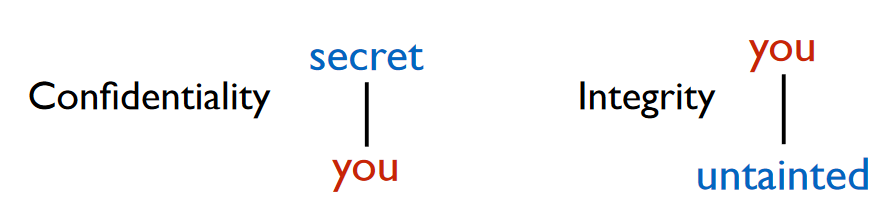
\includegraphics[scale=0.4]{1.png}
\end{figure}
We want to ensure that propagation of information by programs respects information flow policies, i.e. there are no illegal flows. This means an attacker cannot infer secret input or affect critical output by inserting inputs into the system and observing its outputs.

\section{Noninterference}
\subsection{Definition}
A program is secure if, for every observational level $L$, for any two runs of the program that are given the same low inputs, if the program terminates in both cases, then it produces the same low outputs.
\subsection{Attackers}
\subsubsection{Concurrent Attacker}
An attacker program that is concurrently composed with the observed program does not depend on its termination. It has access to "low" outputs, and possibly non-termination (or even intermediate steps). Considering the following programs:
\begin{itemize}
\item $p_L$="$file_L$"; if RUID access to $p_L$ then $f$=open($p_L$);$f=0$ (has RUID=$L$ and EUID=$H$)
\item $p_L = file_H$
\end{itemize}
Both are safe according to our notion of noninterference, but when composed concurrently, the program is insecure.\\
\\
Possibilistic Input-Output Noninterference: is sensitive to whether the program is capable of terminating and producing certain final outputs.
\subsubsection{Intermediate-Step Attacker}
\begin{itemize}
\item $x_L := y:H ; x_L := 1$
\end{itemize}
Possible low outcomes do not depend on $y_H$. However, the intermediate steps differ.\\
\\
Intermediate-step-sensitive Noninterference: is sensitive to intermediate steps of computations.
\subsubsection{Time-Sensitive Attacker}
\begin{itemize}
\item $x_L:=0$ ; if $y_H$ then skip else skip;skip;skip;skip ; $x_L:=1$
\end{itemize}
Possible outcomes and intermediate steps do not depend on $y_H$. However, the time it takes to change the value of $x_L$ is different.\\
\\
Temporal Noninterference: is sensitive to the time it takes to produce outputs.
\subsubsection{Probabilistic Attacker}
\begin{itemize}
\item $x_L := y_H$ || $x_L$ := random(100)
\end{itemize}
Possible outcomes do not depend on $y_H$. However, the probability of the value of $x_L$ revealing that of $y_H$ is higher.\\
\\
Probabilistic Noninterference: is sensitive to the likelihood of outputs.
\subsection{Downgrading}
Noninterference is simple and provides strong security guarantees. But sometimes we need to leak information in a controlled way.
\begin{itemize}
\item Declassification (for confidentiality)
Example: flow declarations locally enable more flows
\begin{figure}[H]
\centering
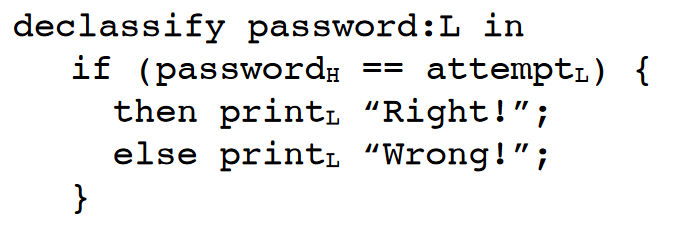
\includegraphics[scale=0.5]{3.png}
\end{figure}
\item Endorsement (for integrity)
Example: pattern matching in Perl’s taint mode
\begin{figure}[H]
\centering
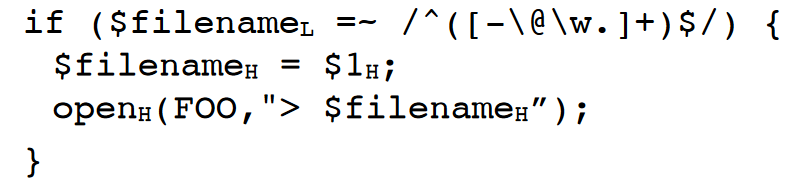
\includegraphics[scale=0.5]{4.png}
\end{figure}
\end{itemize}
\section{Formal Semantics}
We will use two techniques to define the semantics of a programming language:
\begin{itemize}
\item Denotational semantics for expressions: defines mathematically what is the result of a computation.
\item Operational semantics for instructions: describes how the effect of a computation is produced when executed on a machine
\end{itemize}
\subsection{WHILE Language}
This language has the following syntatic categories:
\begin{itemize}
\item $c$: constants
\item $x$: variables
\item $a$: arithmetic expressions
\item $t$: tests
\item $S$: statements
\end{itemize}
And follows the grammar:
\begin{itemize}
\item Operations: $op:: = + | - | \times | /$
\item Comparisons: $cmp ::= < | \leq | = | \neq | \geq | >$
\item Expressions: $a::= c | x | a_1 \; op \; a_2$
\item Tests: $t ::= a_1 \; cmp \; a_2$
\item Statements: $S ::= x:=a | skip | S_1; S_2 | if \; t\; then \; S \; else \; S | while \; t \; do \; S$
\end{itemize}
The state/memory is represented as a function that maps variables to integers, $\rho$, for example, $\rho(x) = 1$. Now, we define the following semantic functions:
\begin{itemize}
\item $\mathcal{A}$: function that maps pairs of arithmetic expression and state to integers ($\mathcal{A}(x)_\rho = \rho(x)$)
\item $\mathcal{B}$: function that maps pairs of test and state, to booleans ($\mathcal{B}(a_1 \; cmp \; a_2)_\rho = \mathcal{A}(a_1)_\rho \; cmp \; \mathcal{A}(a_2)_\rho$)
\item $\mathcal{S}$: partial function that maps pairs of statement and state to state ($<S,\rho> \rightarrow \rho'$: when executing program $\mathcal{S}$ on memory $\rho$ we obtain the new memory $\rho$'. $<S,\rho> \rightarrow <\mathcal{S}', \rho'>$: Performing one step of program $\mathcal{S}$ on memory $\rho$ leaves the continuation $\mathcal{S}'$ and produces new memory $\rho$')
\end{itemize}
The list of big-step axioms and rules is as follows:
\begin{figure}[H]
\centering
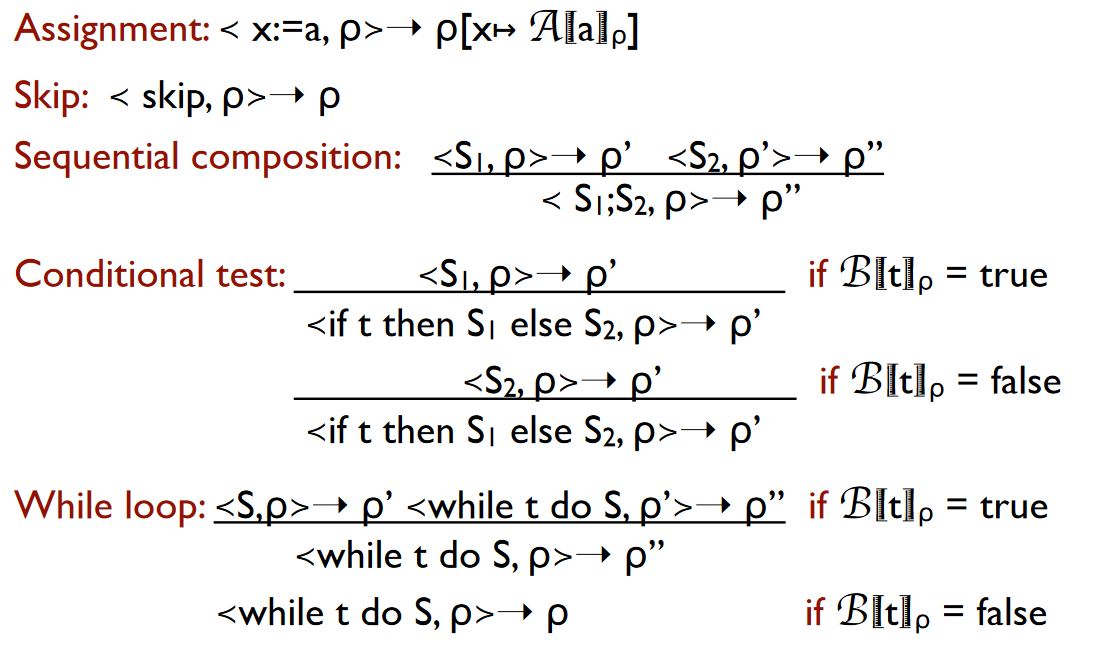
\includegraphics[scale=0.4]{5.png}
\end{figure}
For example, the sequential composition rule could be read as follows: When the first program starting on $\rho$ produces $\rho$' and the second program starting on $\rho$' produces $\rho$'', then  the entire sequential
composition starting on $\rho$ produces $\rho$''. The following is an example of a chaining of these rules:
\begin{figure}[H]
\centering
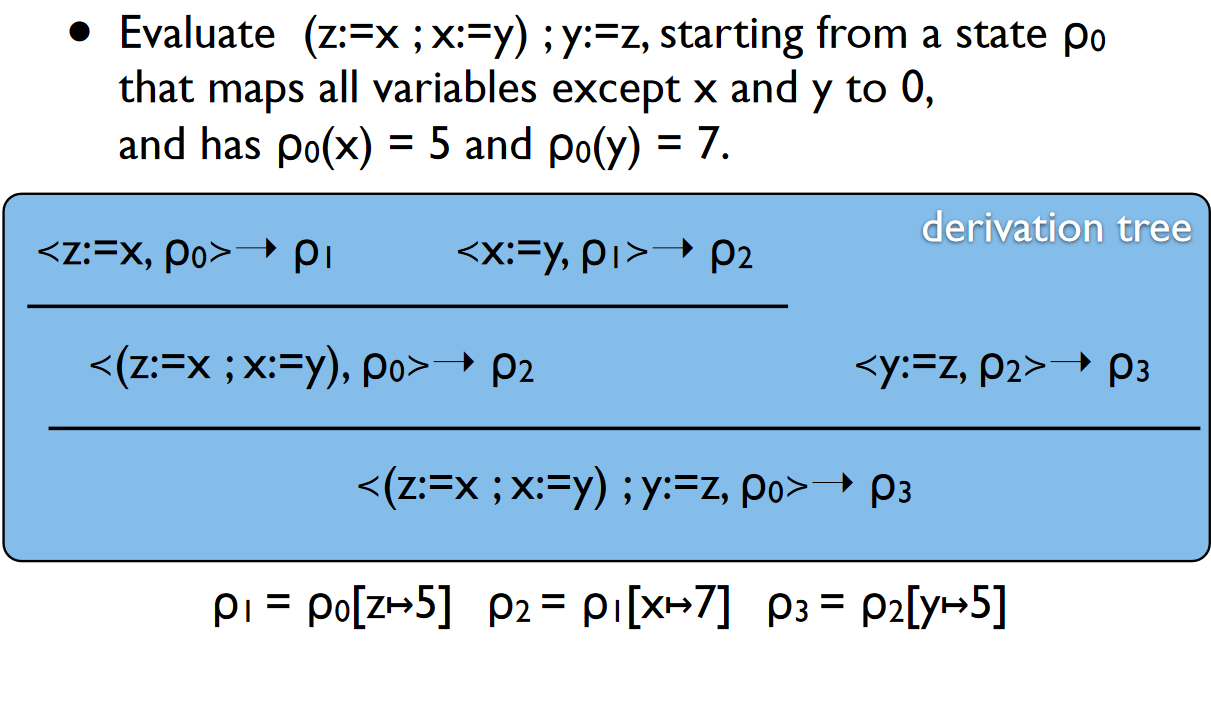
\includegraphics[scale=0.4]{6.png}
\end{figure}
\section{Security Properties and Enforcement Mechanisms}
The definition of a security property is often not enough, since devs make mistakes and understanding whether a program satisfies the property is not always straightforward. At their core, security properties are about behaviour:
\begin{itemize}
\item Functional correctness
\item Robustness
\item Safety
\item ...
\end{itemize}
Enforcement mechanisms were created to this end, automating the algorithm of preventing any given program from performing "unwanted" behaviors.
\subsection{Program Analysis}
Program analysis is the process of automatically analyzing the behavior of computer programs. The main aims of program analysis are:
\begin{itemize}
\item Optimization - about performance, to compute in a more efficient way
\item Correctness - about assurance, to compute as intended
\end{itemize}
Automatic analysis can give stronger guarantees in less time, but is limited in scope and precision, which may come in the form of false positives or negatives.\\
\\
Security properties typically talk about behavior of programs, and are often undecidable. On the other hand, enforcement mechanisms provide an automatic way of accepting/rejecting the behavior of programs, and are expected to be decidable.
\subsubsection{Timing of Program Analysis}
Program analysis may be done before program execution (static), during execution (dynamic) or using a combination of both, using the output of one to another (hybrid).
\subsection{Static Analysis Mechanisms}
Static analysis is closely related to compilation. Some tools used for static analysis include:
\begin{itemize}
\item String matcher: runs directly over source code. Simple tools like grep and findstr can do a very basic form of analysis.
\item Lexical analyzer: runs over the tokens generated by the scanner. Can look for dangerous library/system calls.
\item Semantic analyzers:
\begin{itemize}
\item Control flow analysis:  performs checks based on the possible control paths of a program; used to verify  properties that depend on the sequencing of instructions.
\item Data-flow analysis: gathers information about the possible set of values calculated at various points of a program.Can determine where an actual value assigned to a variable might propagate.
\item Type checking: associate types to selected programs that fulfill certain requirements (eg. are considered correct with respect to a property)
\end{itemize}
\end{itemize}
\subsubsection{Interactive Analysis}
Verification of complex properties can be achieved with more human intervention, such as model checking or program verification.
\begin{itemize}
\item Model checking: checks a model (description) of a program, or the code itself. Enables to check its design.
\item Program Verification: formally proves a property about a program. Uses a specification language (program logic) for expressing properties of a program and an associated logic for (dis)proving that programs meet specifications.
\end{itemize}
\subsubsection{Static analysis for Information Flow}
\begin{enumerate}
\item Definition of the language
\item Information flow policy of security levels
\item Classification of objects into security levels
\item Security property of programs
\item Mechanism for selecting secure programs
\item Guarantees about the mechanism
\end{enumerate}

\chapter{Vulnerabilites And Secure Software Design}
In secure software design, there are 3 main security attributes: confidentiality, integrity and avaliability.
\section{Vulnerabilities}
A vulnerability is a system defect relevant security-wise, which may be exploited by an attacker to subvert security policy. Vulnerabilities may be classified as:
\begin{itemize}
\item Design vulnerabilities
\item Coding vulnerabilities
\item Operational vulnerabilities
\end{itemize}
\section{Attacks}
Attacks enter through interfaces, the attack surfaces. Attacks can be techincal or through social engineering, directed or not, manual or automated.
\subsection{Manual Attacks}
Some examples of manual attacks include:
\begin{itemize}
\item Footprinting
\item Scanning
\item Enumeration
\item Discovering vulnerabilites
\item ...
\end{itemize}
\subsection{Automated Attacks}
\subsubsection{Worm}
A worm is composed of a target selector, a scanning motor, a warhead (exploit code), a load and a propagation motor.
\subsubsection{Drive-by Download}
Performed by web pages with malware. When user accesses one with a vulnerable browser, the malware exploits the vulnerability.
\subsubsection{Viruses and Trojans}
Viruses are similar to worms but propagate with physical contact (usb drives, disks, ...). Trojans are also similar but requires the user to run an infected program (e.g. emails with attachments).
\subsection{Torpig}
Torpig is a sophisticated malware. It infects bots with drive-by download. Attackers modify legitimate but vulnerable server for some webpages to request JavaScript code from the attacker’s web server:
\begin{itemize}
\item[1] The victim’s browser accesses the vulnerable server
\item[2] JavaScript code exploits the browser/plugins/etc.
\item[3-4] If an exploit is successful, the script downloads and installs the Mebroot rootkit
(replaces Master Boot Record) – victim becomes a bot. Mebroot has no attack capacity.
\item[5] Contacts C\&C server to obtain malicious modules and stores them encrypted in directory system32 and changes the names and timestamps to avoid suspicions.\\
Every 2h contacts C\&C server: sends its configuration (type/version of modules); gets updates; communication is encrypted over HTTP
\item[6] Every 20 minutes contacts C\&C to upload stolen data
\item[7] When victim visits domain from a list (e.g., a bank), the bot contacts an injection server. Injection server returns attack data: URL of trigger page in the legitimate domain (typ. the login page), where to send results, etc.\\
When user visits trigger page, Torpig asks injection server for another page (e.g., that asks for credit card number)
\end{itemize}
\begin{figure}[H]
\centering
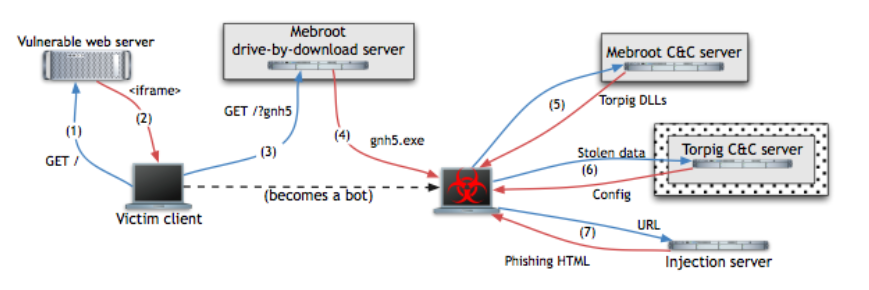
\includegraphics[scale=0.5]{2.png}
\end{figure}
\section{Protection in Operating Systems}
Protection is emplyed to ensure that objects are not accessed by unauthorized subjects. There are two aspects: separation and mediation.
\subsection{Separation}
Common operating systems (Unix, Windows) run software basically in two modes, enforced by the CPU:
\begin{itemize}
\item Kernel mode: software can play with any system resource (memory, I/O devices,...)
\item User mode: access to resources is controlled by the OS. Software has to call the OS kernel to make privileged
operations
\end{itemize}
There are several forms of separation:
\begin{itemize}
\item Physical separation: different processes use different devices (e.g. printers for different levels of security)
\item Temporal separation: processes with different security requirements are executed at different times
\item Logical separation: processes operate under the illusion than no other processes exist
\item Cryptographic separation: processes use cryptography to conceal their data and/ or computations in a way that they become unintelligible to other processes
\end{itemize}
\subsubsection{Memory Protection}
Logical separation is often used to achieve memory protection. The most common solutions are segmentation (program is split in pieces with logical unit, such as code, data, stack...) and paging (program is divided in pages of the same size).\\
\\
From a protection point of view, pages are similar to segments: a process can only  access a segment only if appears in its segment translation table or can only see a page if it appears on its table.
\subsection{Access Control}
Access control is concerned with validating the access rights of subjects to resources of the system. It should be implemented by a reference monitor, following 3 principles:
\begin{itemize}
\item Completeness: it must be impossible to bypass
\item Isolation: it must be tamperproof
\item Verifiability: it must be shown to be properly implemented
\end{itemize}
Some basic access control mechanisms include:
\begin{itemize}
\item Access control lists (ACLs): Each object is associated with a list of pairs (subject, rights)
\item Capabilities: Each subject has a list of objects that it may access, i.e. pairs (object, rights). Capabilities are cryptographically protected against modification and forging
\item Access control matrix: A matrix with lines per subject, columns per object, rights in the cells
\end{itemize}
There are also two basic access control policies:
\begin{itemize}
\item Discretionary Access Control (DAC): access policy defined by the user
\item Mandatory Access Control (MAC): access policy defined by an administrator
\end{itemize}
\subsubsection{Unix Access Control}
Each user in Unix has a username and a user ID (UID). Users can also belong to one or more groups, each with a group ID (GID). Objects (such as files or directories) have an owner identified by a real UID and a real GID. Access permissions are set for the owner, group, and others (world), with read (r), write (w), and execute (x) permissions.\\
\\
When processes interact with objects, their effective UID and effective GID are used to determine access permissions. The kernel compares the effective UID and GID with the permissions of the object to decide whether to grant or deny access.\\
\\
The setuid and setgid bits are additional permission bits that can be set on executable files. When the setuid bit is set on an executable file, the program is executed with the effective UID of the file's owner. Similarly, when the setgid bit is set, the program is executed with the effective GID of the file's group owner. Programs with setuid and owner UID 0 (root) are potential targets for privilege escalation attacks because they may execute with elevated privileges, providing an opportunity for attackers to exploit vulnerabilities.
\section{Race Conditions}
Race conditions violate the assumption of atomicity. The vulnerability lies in a problem of concurrency or lack of proper synchronization. There are several sources of races:
\begin{itemize}
\item Shared data (files and memory)
\item Preemptive routines (signal handlers)
\item Multi-threaded programs
\end{itemize}
There are 3 main kinds of race conditions, discussed next.
\subsection{TOCTOU}
TOCTOU stands for "time-of-check to time-of-use". It is often perpetrated through the use of symbolic links (special files that reference other files/folders).\\
\\
The $access$ function is specially vulnerable as it was designed for $setuid$ programs. It does privilege check using the process’ real UID instead of the effective UID.\\
\\
When a call with a pathname is done ($open, access, stat, lstat, ...$), the pathname is resolved until the inode is found, so if two calls are made one after the other the path can lead to different inodes. The solution is to  avoid the two sequential resolutions by avoiding using filenames inside the program. Functions such as $fstat, fchmod$ and $fchown$ are safe.
\subsection{Temporary Files}
Temporary files have the added problem of being in a shared directory. The typical attack is as follows:
\begin{itemize}
\item Privileged program checks that there is no file X in /tmp
\item Attacker races to create a link called X to some file, say/etc/passwd
\item Privileged program attempts to create X and opens the attacker’s file doing something undesirable that its privileges allow
\end{itemize}
One may use the $mkstemp$ function to create a unique, currently unused, filename from template ($mkdtemp$ for directories).\\
\\
Possible solutions include setting $unmask$ appropriately  and using $fopen$ instead of $open$.
\subsection{Concurrency and Reentrant Functions}
In the previous cases, concurrency is created by the attacker, with malicious intention. In many cases in which there is normal concurrency of operations on objects, operations may have to be executed atomically (using mutual exclusion mechanisms).\\
\\
A function is reentrant if it works correctly even if its thread is interrupted by another thread that calls the same function. Such functions cannot use static variables, global variables, other shared resources like libraries (i.e and can only call other reentrant functions.\\
\\
In some cases, unix signals may be useful in indicating asynchronous events to a process.

\section{Web Application Vulnerabilities}
Web suffers from all the 3 causes of trouble: complexity, extensibility, connectivity.
\subsection{Cross Site Scripting (XSS)}
XSS allows attacker to execute script in the victim’s browser. There are different types of XSS:
\begin{itemize}
\item Reflected XSS (or non-persistent): page reflects user supplied data directed to the user’s browser
\begin{figure}[H]
\centering
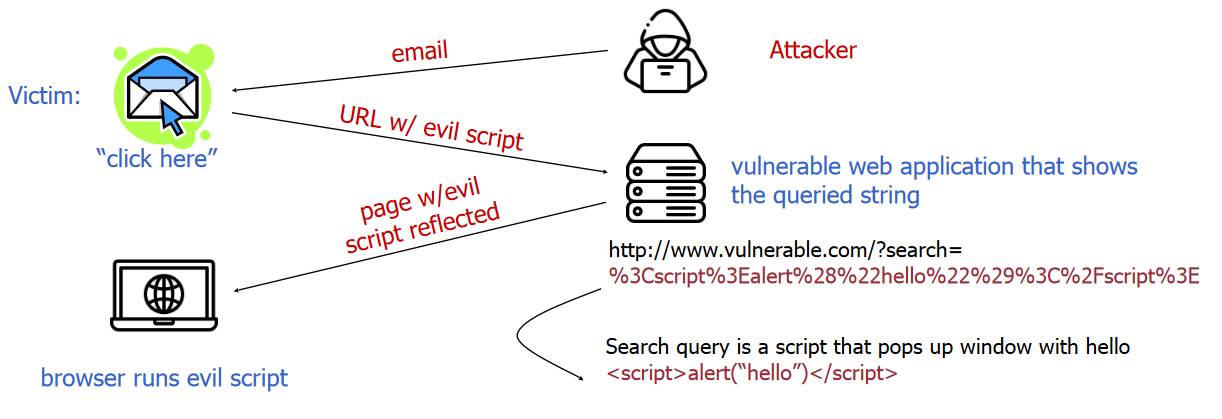
\includegraphics[scale=0.4]{7.png}
\end{figure}
\item Stored XSS (or persistent): hostile data (script) is stored in a database, file, etc., and is later sent to user’s browser
\begin{figure}[H]
\centering
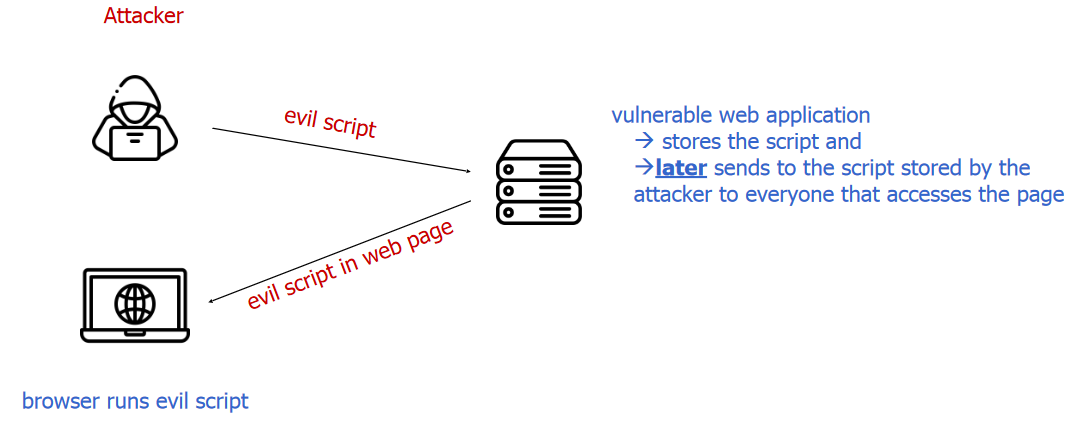
\includegraphics[scale=0.4]{8.png}
\end{figure}
\item DOM based XSS (Document Object Model): manipulates JavaScript code and attributes instead of HMTL
\end{itemize}
In reflected and stored XSS the server injects the script. In DOM based XSS, the client injects the script.\\
\\
Some protection mechanisms are:
\begin{itemize}
\item Server-side input validation
\item Strong output encoding
\item Content Security Policy (level 2)
\item State tracking mechanisms
\end{itemize}
\subsection{CRLF Injection}
It is similar to reflected XSS but the injection is in the response header, while in reflected XSS the injection is in the responde body.\\
\\
The attacker inserts a carriage return (CR) and a life feed (LF) creating a new field in the header, or a second response (HTTP response splitting).\\
\\
Just as in the reflected XSS, the attacker sends the victim a URL of a vulnerable website.
\subsection{Direct Object Reference}
Occours when a site exposes a reference to an internal object and no proper access control (e.g. files, database records, keys, ...).\\
\\
Should be prevented by forbidding the exposure of object references and by doing proper access control.
\subsection{Cross Site Request Forgery (CSRF)}
Many sites do certain actions based on an automatically submitted, fixed, ID, typically a session cookie. The attack consists of forcing the user to execute unwanted actions in a vulnerable site in which it is authenticated. Can be done by sending a link by email or chat.\\
\\
The solution is similar to XSS, but may also consist on using nonces or requiring re-authentication for critical actions.
\subsection{Security Misconfiguration}
Misconfiguration vulnerabilities can exist at any level (OS, web/app server, ...). An attacker can access several things to gain unauthorized access to or knowledge of the system.\\
\\
Protection consists of deploying automated scanners  for detecting missing patches, misconfigurations, use of default accounts, unnecessary services, etc.
\subsection{Failure to Restrict URL Access}
Pages that are "protected" simply by being inaccessible from the "normal" web tree. The attack consists of forced browsing: guess links and brute force to find unprotected pages.\\
\\
Protection relies in having good access control, no "hidden" pages as a form of protection.
\subsection{Unvalidated Redirects and Forwards}
Applications frequently redirect users to other pages. Sometimes the target page is specified in an unvalidated parameter, allowing attackers to choose the destination page.
\subsection{Insecure Cryptographic Storage}
Can be cause by sensitive data not being encrypted, use of home-grown or weak algorithms, ...
\subsection{Insecure Transport Layer Protection}
Sensitive traffic or authenticated sessions may be unencrypted. HTTPS should be used.

\section{Database Vulnerabilities}
SQL injection is the most common vulnerability in modern database systems. It may occour when user input is pasted into SQL commands; the concrete syntax is dependent on the specific DBMS and server-side language used. The steps of an attack include:
\begin{itemize}
\item Identifying parameters vulnerable to injection
\item Database fingerprinting (discover type and version using queries)
\item Discovering DB schema
\item Extracting/adding/modifying data from the DB
\item Denial of service
\item Evading detection
\end{itemize}
\subsection{Methods}
\subsubsection{Tautologies}
Inject code in 1 or more conditional statements so that it always evaluate to true (a tautology). It is commonly used to bypass authentication and extract data.\\
\\
For example: $' \; or \; 1=1 \; -- $. Such an input may be evaluated as: $$SELECT \; accounts \; FROM \; users \; WHERE \; login='' \; or \; 1=1 \; -- \; ' \; AND \; pass='' \; AND \; pin=$$
Commenting the last part and breaking the query.
\subsubsection{Union Query}
Trick the app into returning additional data by injecting $UNION \; SELECT  \; <rest>$. The attacker uses $<rest>$ to extract data from another table, since the query returns the union of data.
\subsubsection{Piggy-Backed Queries}
It does not modify a query, instead adds more queries; requires the DB to be configured to accept multiple statements in a single string.\\
\\
For example: $';DROP \; TABLE \; users\;--$.
\subsubsection{Stored Procedures}
The injection could instead target a stored procedure.
\begin{figure}[H]
\centering
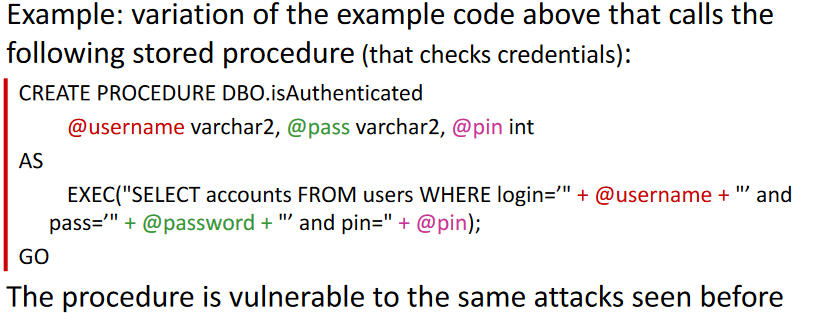
\includegraphics[scale=0.4]{9.png}
\end{figure}
\subsubsection{Illegal/Incorrect Queries}
Find injectable parameters (DB type/version, schema) by causing errors:
\begin{itemize}
\item Syntax errors: identify injectable parameters
\item Type errors: deduce data types of certain columns or extract data
\item Logical errors: reveal names of tables and columns that caused error
\end{itemize}
\subsubsection{Inference}
Attack attempts to infer if a certain condition on the state of the DB is true or false. The objective is similar to using illegal/incorrect queries. There are two techniques:
\begin{itemize}
\item Blind injection: Information is inferred by asking true/false questions
\begin{figure}[H]
\centering
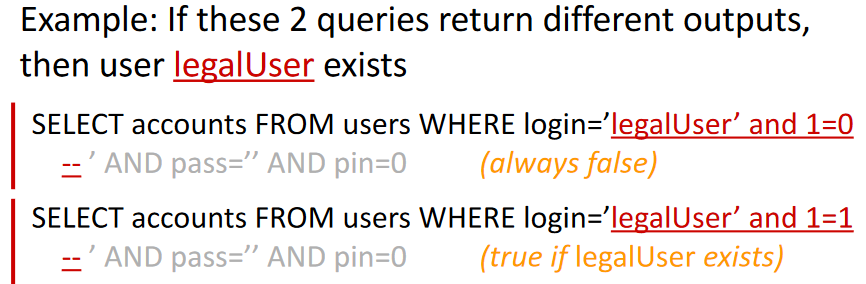
\includegraphics[scale=0.4]{10.png}
\end{figure}
\item Timing attack: Information is inferred from delay in the response, usually with a branch that executes a $WAITFOR$ $DELAY$
\begin{figure}[H]
\centering
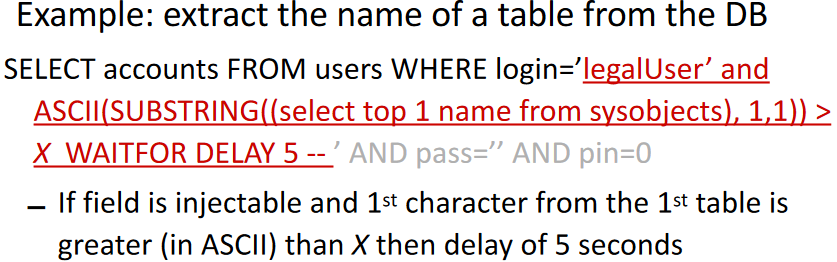
\includegraphics[scale=0.4]{11.png}
\end{figure}
\end{itemize}
\subsubsection{Alternate Encodings}
Not a full attack but a trick to evade detection. The idea is to encode input in an unusual format, such as hex, ascii or unicode. For example: 
$$
SELECT \; a \; FROM \; u \; WHERE \; login='legalUser';exec(char(0x73687574646f776e))\; --\; AND\; ...
$$
In this case it executes as $exec(shutdown)$.
\subsection{Injection mechanisms}
\begin{itemize}
\item GET/POST inputs
\item Cookies (can be used by the server to build SQL commands, $SELECT \; ... \; WHERE \; cookie='\%s'\; ...$)
\item Header fields (in PHP). Replace the $XXX$ in $\$\_SERVER['HTTP\_XXX']$ with $HTTP\_URL$, $HTTP\_ACCEPT\_LANGUAGE$, ...
\end{itemize}
It's also possible to use second-order injection, where the input is provided so that it is kept in the system and later used. For example, registering a new user as $admin'--$; The site correctly escapes the input and accepts it, but will act as an injection on further queries.
\subsection{More Vulnerabilities}
There exist more, less frequent, vulnerabilities in DBMS', such as:
\begin{itemize}
\item Blank and default passwords
\item Unprotected communication (client-server)
\item Several open ports
\item Default (privileged) accounts
\item Code vulnerabilities
\item Encryption problems
\end{itemize}
\section{Data Validation}
There are 3 facets to validation: type, length and syntax. Validation is also tied to integrity checking and business rule enforcing.\\
\\
The first problem that arises is where to perform validation:
\begin{itemize}
\item $1^{st}$ principle: data validation has to be made whenever data crosses a trust boundary
\item $2^{nd}$ principle: there has to be a small set of well defined chokepoints where validations are done
\end{itemize}
\subsection{White and Black Listing}
White listing refers to accepting known good and black listing to rejecting known bad. Of the two, only white listing should be used, since black listing  violates principle of fail-safe defaults.
\subsection{Sanitization}
Sanitization consists of eliminating or encoding characters to make input safe.
\subsubsection{Canonical Representation}
Metacharacter evasion has to be solved by doing canonicalization before validation. For example, $\%64elete$ in canonical form becomes $delete$.\\
\\
Web canonicalization issues are important due to many ways to encode the same character (ascii, UTF, URL encoding)\\
\\
The principle is to do before validation the same decodings the application + interpreter might do after validation (in the same order). For example, if the input comes from URL and is used in UTF-8 in a web page:
\begin{itemize}
\item Decode URL encoding (i.e., hexadecimal escapes, e.g., \%20) to UTF-8
\item Canonicalize UTF-8 char
\item Validate
\end{itemize}
\subsection{Encoding}
Encoding is an alternative/complement to validation. It consists of encoding characters for protection, with the objective of neutralizing dangerous characters (typically metacharacters).
\begin{figure}[H]
\centering
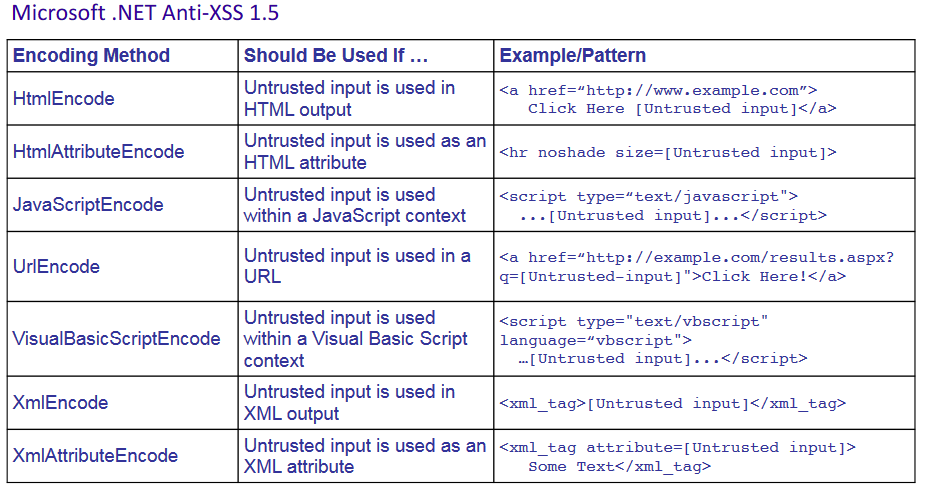
\includegraphics[scale=0.4]{12.png}
\end{figure}

\section{Input Validation}
Trust can be misplaced when there is interaction (i.e. input).\\
\\
One example of input are environment variables. The libraries used by the program may not do enough sanity checking of the environment variables, such as PATH and IFS.
\subsection{Metadata and Metacharacters}
Data is often stored with metadata, which can be represented:
\begin{itemize}
\item In-band: as part of the data, e.g., strings in C (a special character is used to indicate the termination)
\item Out-of-band: separated from data, e.g., strings in Java (the number of characters is metadata stored separately from the characters)
\end{itemize}
In-band metacharacters are a source of many vulnerabilities. They occur because the program trusts input to contain only characters, not metacharacters. The most typical attacks using metacharacters are:
\begin{itemize}
\item Embedded delimiters ($\backslash$n)
\item NUL character injection ($\backslash$0)
\item Separator injection (;)
\end{itemize}
\subsection{Format String Vulnerabilities}
Format strings are used in C, in functions of the families $printf$, $err$ and $syslog$. They are vulnerable because the parameters passed are put in the stack before the function is called. If the format string is controlled by an attacker it might be used to crash the program, print arbitrary memory addresses or write arbitrary values in memory.\\
\\
The solution is simple: always write the format string in the program.

\section{Buffer Overflows}
A buffer is a memory space with contiguous chunks of the same data type (typically bytes or chars).We have a buffer overflow when a program writes after the end of a buffer.\\
\\
When a buffer overflow occours, the program becomes unstable, and may crash or proceed. Side effects depend on how much data was written (or overwritten), if the program tries to read such data, etc.
\subsection{Prevention}
The prevention method is simple: always do bounds checking; problems might arise only when you cannot control input. Some C functions should be avoided:
\begin{itemize}
\item $gets$
\item $strcpy$
\item $sprintf$
\item $scanf$
\item $streadd$
\item ...
\end{itemize}
There is also a risk of internal BOs, when the overflow is not in the program’s buffers but inside a library function.
\subsection{Stack Overflows}
\subsubsection{Stack Smashing}
Stack smashing is the classic stack overflow attack. For example, the following code is vulnerable, since is inserts untrusted input in $buf$ without checking:
\begin{figure}[H]
\centering
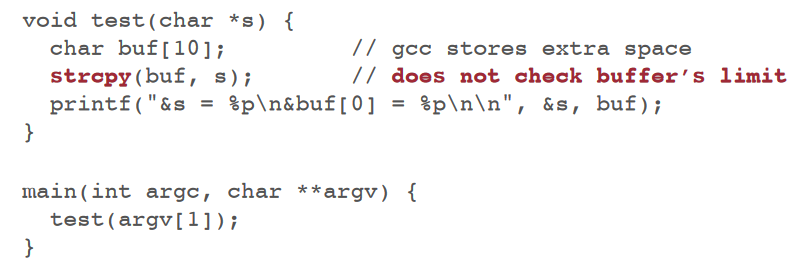
\includegraphics[scale=0.4]{13.png}
\end{figure}
Such attacks can overflow local vars or the saved EIP, and may crash or modify the state of the program, as well as executing code. The effect on the stack can be visualized on the following image:
\begin{figure}[H]
\centering
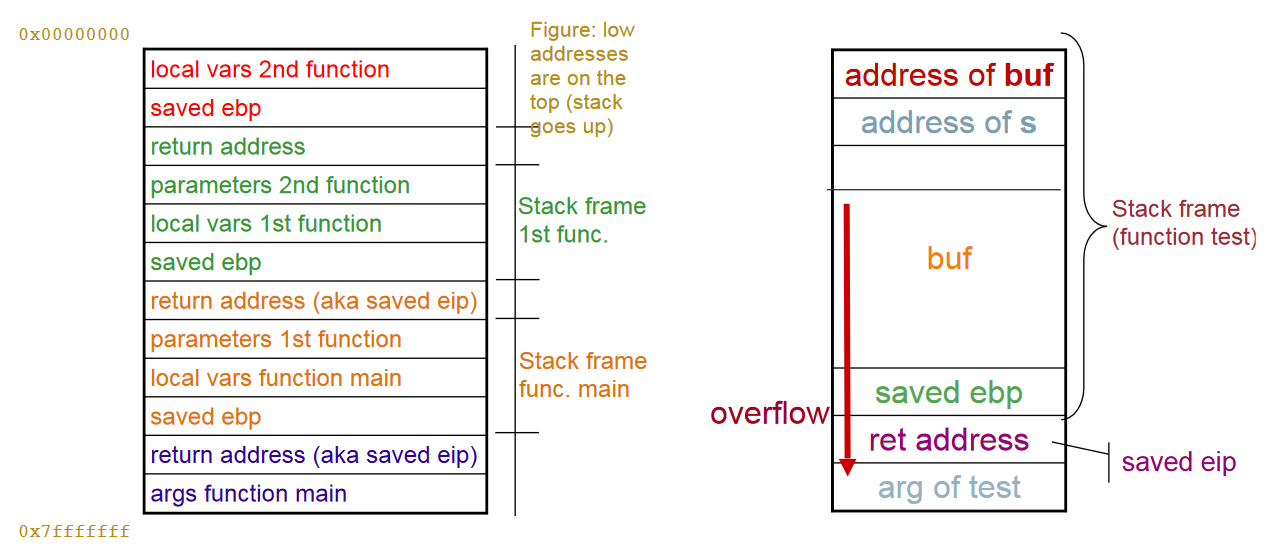
\includegraphics[scale=0.4]{14.png}
\end{figure}
\subsubsection{Code Injection}
Consists of inputting arbitrary code to be executed. For this attack, the stack has to be executable and the address where the code is injected has to be discover. It is often difficult because of the reduced space and the inclusion of null bytes (functions like $strcpy$ stop in the first zero).
\subsubsection{Arc Injection / return-to-libc}
Consists of inserting a new arc in the program control-flow graph (stack-smashing includes a new node in the graph). For example, overrun the return address to point to code already in the program.
\subsubsection{Pointer Subterfuge}
Pointer subterfuge is a general term for exploits that involve modifying a pointer. The objective can be to circumvent protections against BOs when the return address is protected. There are four types:
\begin{itemize}
\item Function-pointer clobbering: modify a function pointer to point to attacker supplied code
\item Data-pointer modification: modify address used to assign data
\item Exception-handler hijacking: modify pointer to an exception handler function
\item Virtual pointer smashing modify the C++ virtual function table associated with a class
\end{itemize}
\section{Dynamic Protection}
The idea is to block attacks that may exploit existing vulnerabilities, mostly the case of memory corruption attacks.
\subsection{Canaries}
Canaries may be used to detect some stack smashing attacks. They do not detect BO attacks that modify local variables, as those are above the canary, but detect (altough possibly too late) BO attacks againts the function arguments (these are below the ret address).
\begin{figure}[H]
\centering
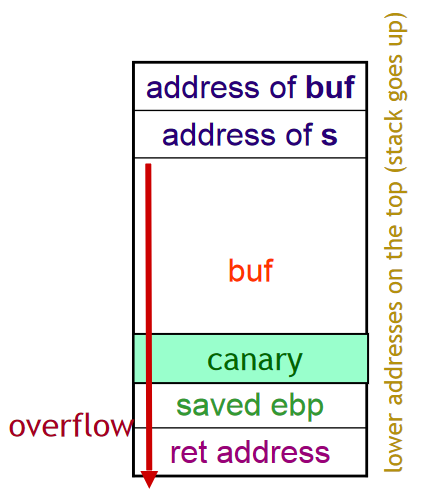
\includegraphics[scale=0.4]{15.png}
\end{figure}
In order to allow canaries to protect local vars from overflows, a simple solution consists of reordering the stack layout, placing the local vars between the buffer and canary.\\
\\
To allow the protection of function arguments, some compilers put the args in CPU registers, preventing this attack. An alternate solution consists of copying the args to the top of the stack in the beginning of a function.
\subsection{Non-executable Stack and Heap}
Many buffer overflow attacks involve injecting shell code in the stack/heap. A simple protection is to mark these memory pages as non-executable.
\subsection{Randomization and Obfuscation}
\subsubsection{Address Space Layout Randomization (ASLR)}
ASLR is efective against most BO attacks, but not those against local variables. The idea is to randomize the addresses where code and data are placed in runtime. What is randomized are not the physical addresses by shuffling pages around the RAM (which always happens anyway), but the logic/linear addresses, i.e., the organization of the virtual memory of a process.
Altough this does not prevent exploitation, it makes it unreliable and harder. Only some elements can be randomized:
\begin{itemize}
\item Code: addresses where apps and dynamic libraries are loaded
\item Stack: starting address of the stack of each thread
\item Heap: base address of the heap
\end{itemize}
\subsubsection{Instruction Set Randomization}
Code injection would be almost impossible if each computer had its own random instruction set. With this approach, legitimate code is scrambled and malicious code is not, hopefully making it possible to execute.\\
\\
A practical case would be SQL  instruction randomization to avoid SQL injection.
\subsubsection{Function Pointer Obfuscation}
Long-lived function pointers are often the target of memory corruption exploits, as they provide a direct method for seizing control of program execution.\\
\\
Pointer obfuscation mitigates this problem. The idea is to XOR the pointer with a random secret cookie, keeping it protected when not needed.
\subsection{Integrity Verification}
\subsubsection{Windows Structured Exception Handling (SEH)}
This feature is present in Windows operating systems. When an exception is generated, Windows examines a linked list of $EXCEPTION\_REGISTRATION$ structures in the stack. Such structures include pointers to the handlers, which  can be overrun and an exception raised to force a jump to that address.
\subsubsection{Array Bound Checking}
BOs are caused by lack of array bound checking, so doing the check solves the problem. It is already done in languages like Java and supported in C compilers, such as $gcc$, with some restrictions.
\begin{figure}[H]
\centering
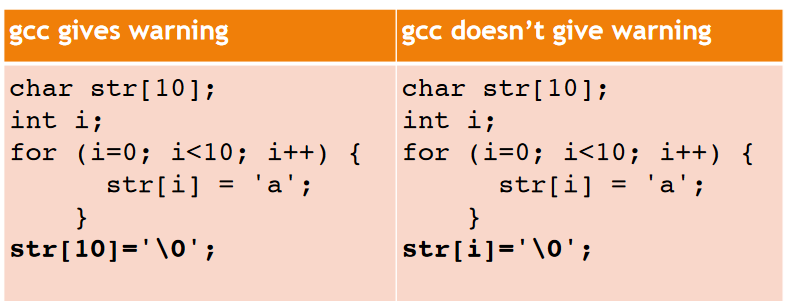
\includegraphics[scale=0.4]{16.png}
\end{figure}
\subsubsection{Detection Through Interception}
$libsafe$ is a library with wrappers for problematic libc functions. When a function is called, the wrapper first checks if the buffer is not being overrun, using EBP as an upper bound.
\subsubsection{Control-flow Integrity}
Stack Shield has a global ret stack:
\begin{itemize}
\item Whenever a function is called, the return address is stored in a $GlobalRetStack$ (besides the normal stack)
\item Before the function returns, check if the return address in the normal stack and the $GlobalRetStack$ match
\end{itemize}
\subsection{Filtering}
\subsubsection{Web Application Firewalls}
WAFs are application-level firewalls for webapps:
\begin{figure}[H]
\centering
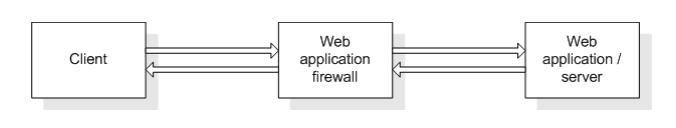
\includegraphics[scale=0.4]{17.png}
\end{figure}
The interposition can be obtained in four ways:
\begin{itemize}
\item Bridge: WAF installed as a transparent bridge (switch)
\item Router: network reconfigured to direct traffic through the WAF
\item Reverse proxy: represents the web server for the clients
\item Embedded: WAF is installed as a web server plug-in
\end{itemize}
The reaction to the detection of an attack can range from blocking the HTTP request, to ending the session and even blocking the user.
\end{document}
% next: LBS 4